\documentclass{beamer}
\usefonttheme[onlymath]{serif}
\usepackage{amsmath}
\usepackage{amsfonts}
\usepackage[export]{adjustbox}
\usepackage[utf8]{inputenc}
\usepackage{tikz} 
\usetikzlibrary{bayesnet}
% definitions
\def\H{\mathcal{H}}
\def\X{\mathbf{X}}
\def\w{\mathbf{w}}
\def\W{\mathbf{W}}
\def\const{\mathrm{const}}
\def\Var{\mathrm{Var}}
\def\tr{\mathrm{tr}}
\def\T{\top}
\def\U{\mathbf{U}}
\def\S{\mathbf{S}}
\def\V{\mathbf{V}}
\newcommand{\argmin}{\mathop{\mathrm{argmin}}}
\newcommand{\argmax}{\mathop{\mathrm{argmax}}}
\newcommand{\minimize}{\mathop{\mathrm{minimize}}}
\newcommand{\maximize}{\mathop{\mathrm{maximize}}}
\newcommand{\st}{\mathop{\mathrm{subject\,\,to}}}
 
%Information to be included in the title page:
\usecolortheme{seahorse}
\title{Latent Dirichlet Allocation}
\author{Kangcheng Hou}
\institute{Zhejiang University}
\date{\today}

    
    
\begin{document}
    
\frame{\titlepage}

\begin{frame}{Introduction}
Here is a PGM of LDA.

\begin{figure}[H]
    \centering
    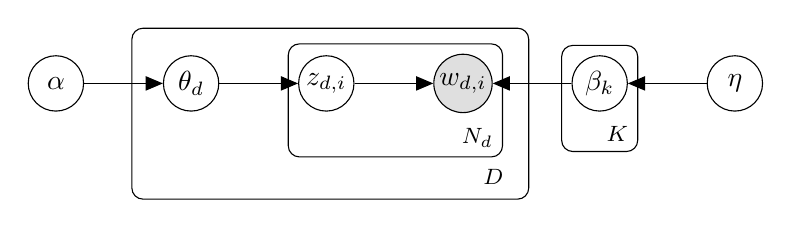
\begin{tikzpicture}
      % Nodes
      % parameters and data
      \node[latent]           (alpha)    {$\alpha$}; %
      \node[latent, right= of alpha]  (theta) {$\theta_d$};
      \node[latent, right= of theta]  (z) {$z_{d,i}$};
      \node[obs, right = of z]  (w) {$w_{d,i}$};
      \node[latent, right = of w]  (phi) {$\beta_k$};
      \node[latent, right = of phi]  (beta) {$\eta$};
      % edges
       \edge{alpha}{theta};
       \edge{theta}{z};
       \edge{z}{w};
       \edge{phi}{w};
       \edge{beta}{phi};
     % Plates
      {
       \tikzset{plate caption/.append style={below=20pt of #1.south east}}
       \plate[inner ysep=7pt, inner xsep=10pt, xshift=-1pt, yshift=2pt] {plate1} {(theta)(z)(w)} {$D$};
      }
    
      \plate[]{plate2}{
        (z)(w)
      }{$N_d$};
    
      \plate[]{plate3}{
        (phi)
      }{$K$};
    \end{tikzpicture}
    \end{figure}
We want to sample the posterior distribution of the latent variable $z_{d,i}$ given $w_{d,i}$. One method is gibbs sampling, in every iteration, we sample $z_i$ from distribution $p(z_i | z_{\neg i}, w)$.
The joint distribution is 
$$p(w,z | \alpha, \beta) = p(w | z, \beta) p(z | \alpha)$$
\end{frame}
\begin{frame}{Posterior predictive of Dirichlet-Multinomial}
Suppose we have dirichlet prior distribution,
$$p(\theta | \alpha) = \text{Dir}(\theta | \alpha) \propto \prod_{k=1}^K \theta_i^{\alpha_i - 1}$$

\end{frame}
\begin{frame}[allowframebreaks]{Joint distribution}
The joint distribution is $p(w,z | \alpha, \beta) = p(w | z, \beta) p(z | \alpha)$. The first part is

$$p(w | z, \beta) = \int_{\phi_{1 : K}} p(w | z, \phi_{1 : K})p(\phi_{1 : K} | \beta)d \phi_{1 :K}$$
Let's see $p(w | z, \phi_{1 : K})$ first, 
$$p(w | z, \phi_{1 : K}) = \prod_{i=1}^W \phi_{z_i, w_i}$$
Or we can rephrase it in another way, where we classify it by topic.
$$p(w | z, \phi_{1 : K}) = \prod_{i=1}^W \phi_{z_i, w_i} = \prod_{k=1}^K \prod_{v=1}^V \phi_{k,v}^{n_k^{(v)}}$$
And $$p(\phi_{1 : K} | \beta) = \prod_{k=1}^K \prod_{v=1}^V \phi_{k,v}^{\beta_v - 1} $$
Adding these two together, we have
$$p(w | z, \beta) = \prod_{k=1}^K \frac{B(n_k + \beta)}{B(\beta)}$$
$n_k$ represents the word apperance frequencies in topic $k$.
The topic distribution $p(z | \alpha)$ can be derived similarly,
$$p(z | \alpha) = \prod_{d=1}^D\frac{B(n_d + \alpha)}{B(\alpha)}$$
So the joint distribution is
$$p(z,w | \alpha, \beta) = \prod_{k=1}^K \frac{B(n_k + \beta)}{B(\beta)}\prod_{d=1}^D\frac{B(n_d + \alpha)}{B(\alpha)}$$
$$p(z_i = k | z_{\neg i}, w, \alpha, \beta) = \frac{p(w,z) | \alpha, \beta}{p(w, z_{\neg i} | \alpha, \beta)} \propto p(w,z | \alpha, \beta) $$
And the multinomial parameters can be derived as follows
$$p(\theta_d | w, z, \alpha) \sim \text{Dir}(\theta_m | n_m + \alpha)$$
$$p(\phi_d | w, z, \beta) \sim \text{Dir}(\phi_d | n_d + \beta) $$
\end{frame}


\end{document}